% vim: set foldmethod=marker foldlevel=0:

\documentclass[a4paper]{article}
\usepackage[UKenglish]{babel}

% NOTE: hyperref has to come before preamble
\usepackage{hyperref}

\usepackage{preamble}

\usepackage{graphicx}
\graphicspath{ {./imgs/} }

\fancyhead[L]{MA144 Assignment 2}
\title{MA144 Methods of Mathematical Modelling 2, Assignment 2}

\begin{document}

\maketitle

\setlength{\parindent}{0em}
\setlength{\parskip}{1em}

% {{{ Q1
\question{1}

\subsection{~}

The heat equation is
$$\pdd ut = \alpha \pddd 2ux$$

A solution to the heat equation is
$$u(x, t) = \f1{\sqrt{2 \pi t}}\, \e^{- x^2 / 2t} = \f1{\sqrt{2\pi}}\, t^{-\f12}\, \e^{- x^2 / 2t}$$

\subsubsection{~}

The solution gives \begin{align*}
\pdd ut &= \f1{\sqrt{2\pi}} \l( t^{-\f12} \e^{-x^2 / 2t} \f{x^2}{2t^2} - \f12 t^{-\f32} \e^{-x^2 / 2t} \r)\\[1ex]
&= \f1{\sqrt{2\pi}}\, \e^{-x^2 / 2t} \l( t^{-\f12} \f{x^2}{2} t^{-2} - \f12 t^{-\f32} \r)\\[1ex]
&= \f1{2\sqrt{2\pi}}\, \e^{-x^2 / 2t} \l( x^2 t^{-\f52} - t^{-\f32} \r)\\[1ex]
&= \f1{2\sqrt{2\pi}}\, \e^{-x^2 / 2t} t^{-\f32} \l( x^2 t^{-1} - 1 \r)\\[1ex]
&= \f1{2\sqrt{2\pi t^3}}\, \e^{-x^2 / 2t} \l( \f{x^2}t - 1 \r)
\end{align*}
and \begin{align*}
\pddd 2ux &= \pdiff x \l( \f1{\sqrt{2\pi t}}\, \e^{-x^2 / 2t} \l( \f{-x}t \r) \r)\\[1ex]
&= \pdiff x \l( \f{-1}{\sqrt{2\pi t^3}}\, x \e^{-x^2 / 2t} \r)\\[1ex]
&= \f{-1}{\sqrt{2\pi t^3}} \l( \e^{-x^2 / 2t} + x \e^{-x^2 / 2t} \l(\f{-x}t\r) \r)\\[1ex]
&= \f1{\sqrt{2\pi t^3}} \e^{-x^2 / 2t} \l( \f{x^2}t - 1 \r)
\end{align*}

Therefore $\alpha = 2$ for this solution.

\subsubsection{~}

$$u(x, 1) = \f1{\sqrt{2\pi}}\, \e^{-x^2 / 2}$$

\begin{figure}[h]
	\centering
	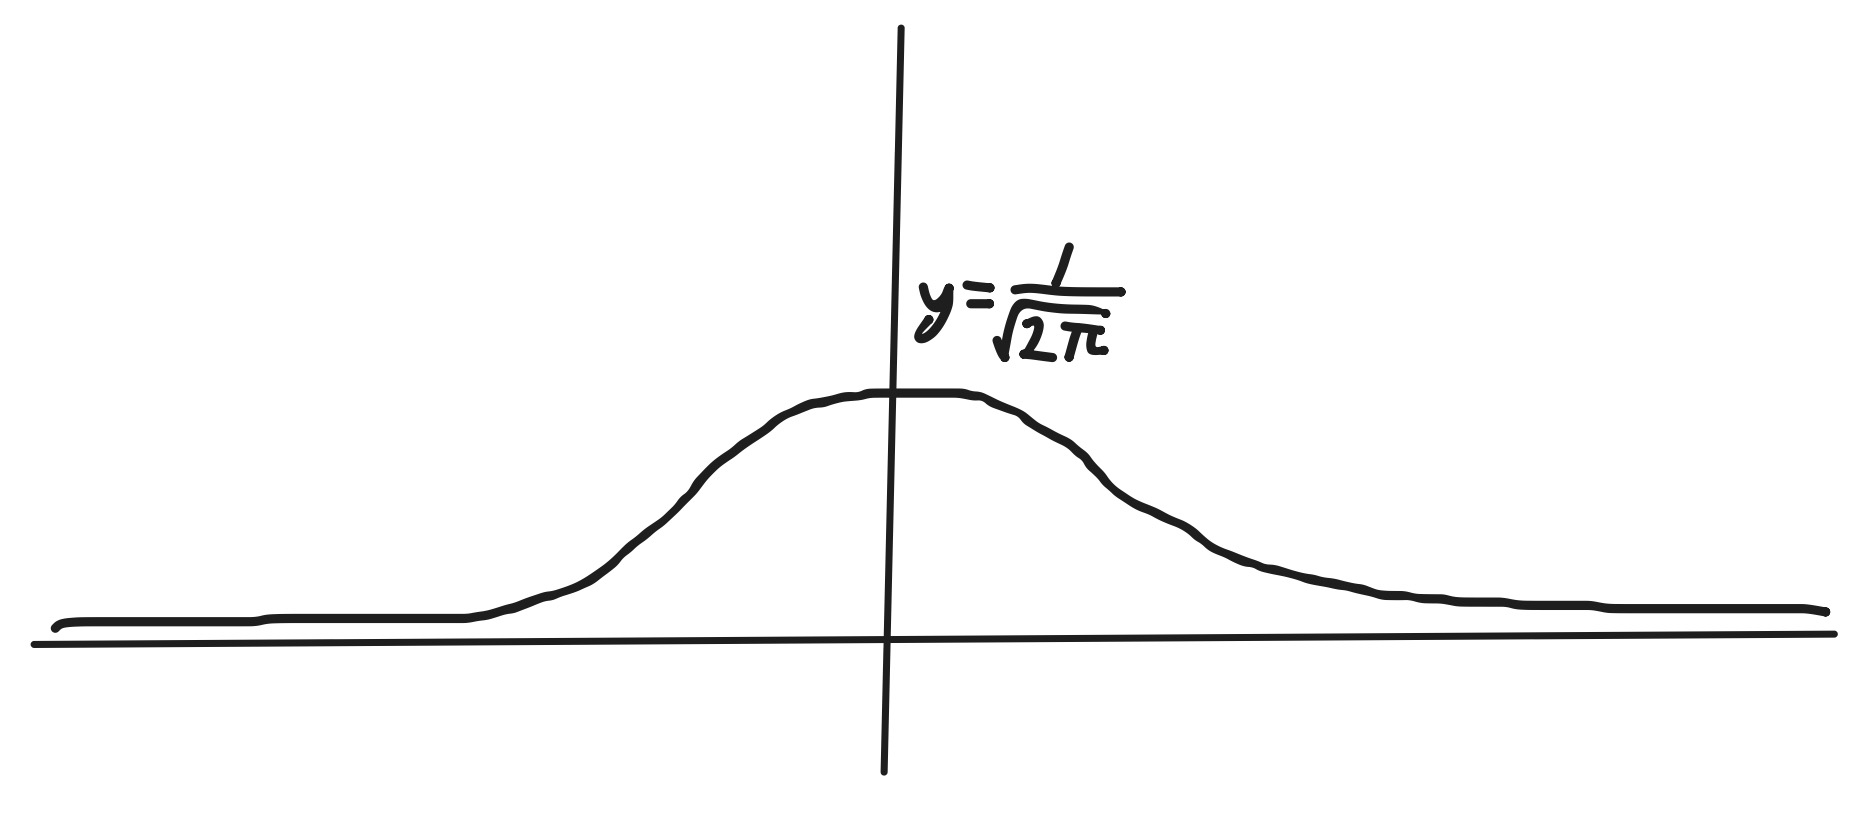
\includegraphics[scale=0.35]{Q1a-ii}
	\caption{A plot of $y = u(x,1)$}
\end{figure}

\subsection{~}

The wave equation is
$$\pddd 2ux = \f1{c^2}\, \pddd 2ut$$

A solution to the wave equation is
$$u(x, t) = \sin x \cos \beta t$$
where $\beta > 0$.

\subsubsection{~}

The solution gives \begin{align*}
\pddd 2ux &= \pdiff x \l( \cos x \cos \beta t \r)\\[1ex]
&= -\sin x \cos \beta t\\[1ex]
&= -u(x, t)
\end{align*}
and \begin{align*}
\pddd 2ut &= \pdiff t \l( -\beta \sin x \sin \beta t \r)\\[1ex]
&= -\beta^2 \sin x \cos \beta t\\[1ex]
&= -\beta^2 u(x, t)
\end{align*}

Plugging this into the wave equation gives $$-u(x, t) = -\f{\beta^2}{c^2} u(x, t)$$
Therefore $\df{\beta^2}{c^2} = 1$ so $\beta = \pm c$. We know $c > 0$ and we want $\beta > 0$, so $\beta = c$.

\subsubsection{~}

Let $u(x, t) = f(x+ct) + g(x-ct)$. Then by the chain rule, \begin{align*}
\pddd 2ux &= \pdiff x \l( f'(x+ct) + g'(x-ct) \r)\\[1ex]
&= f''(x+ct) + g''(x-ct)
\end{align*}
and \begin{align*}
\pddd 2ut &= \pdiff t \l( c f'(x+ct) - c g'(x-ct) \r)\\[1ex]
&= c^2 f''(x+ct) + c^2 g''(x-ct)
\end{align*}

Therefore $\ds \pddd 2ux = \f1{c^2} \pddd 2ut$, so this $u$ satisfies the wave equation.
% }}}

% {{{ Q2
\newquestion{2}

$$f(x, y) = \e^x + y^3 - 2x - 3y$$

\subsection{~}

$$\pdd fx = \e^x - 2 \qquad \pdd fy = 3y^2 - 3$$

Critical points are where $\ds \pdd fx = \pdd fy = 0$. That means $\e^x - 2 = 0$ so $x = \log 2$, and $3y^3 - 3 = 0$ so $y = \pm 1$. Therefore the critical points of $f$ are at $(\log 2, 1)$ and $(\log 2, -1)$.

The Hessian matrix of $f$ is $\begin{pmatrix} \e^x & 0\\ 0 & 6y \end{pmatrix}$ and its determinant is $D = 6 \e^x y$.

At the point $(\log 2, 1)$, $D = 12$ and $f_{xx} = 2$, so this point is a local minimum point.

At the point $(\log 2, -1)$, $D = -12$, so this point is a saddle point.

\subsection{~}

Linear approximation around $P = (0, 2)$ gives \begin{align*}
f(x, y) &\approx f(0, 2) + \l. \nabla f \r|_{(0,2)} \cdot \begin{pmatrix}x\\ y-2\end{pmatrix}\\[1ex]
&= \l( 1 + 8 - 0 - 6 \r) + \l. \begin{pmatrix}\e^x - 2\\ 3y^2 - 3\end{pmatrix} \r|_{(0,2)} \cdot \begin{pmatrix}x\\ y-2\end{pmatrix}\\[1ex]
&= 3 + \begin{pmatrix}-1\\ 9\end{pmatrix} \cdot \begin{pmatrix}x\\ y-2\end{pmatrix}\\[1ex]
&= 3 -x + 9y - 18\\[1ex]
\thf f(x, y) &\approx -15 -x + 9y
\end{align*}

Therefore \begin{align*}
f(0.01, 1.99) &\approx -15 - 0.01 + 9 \times 1.99\\
&= -15.01 + 9 + 8.91\\
&= -15.01 + 17.91\\
&= 2.9
\end{align*}

For completeness, $f(0.01, 1.99)$ is actually around $2.900649$, so this approximation is very good.

\subsection{~}

The direction of steepest descent at point $P$ is $\l. -\nabla f \r|_P = \begin{pmatrix}1\\ -9\end{pmatrix}$.

\begin{figure}[h]
	\centering
	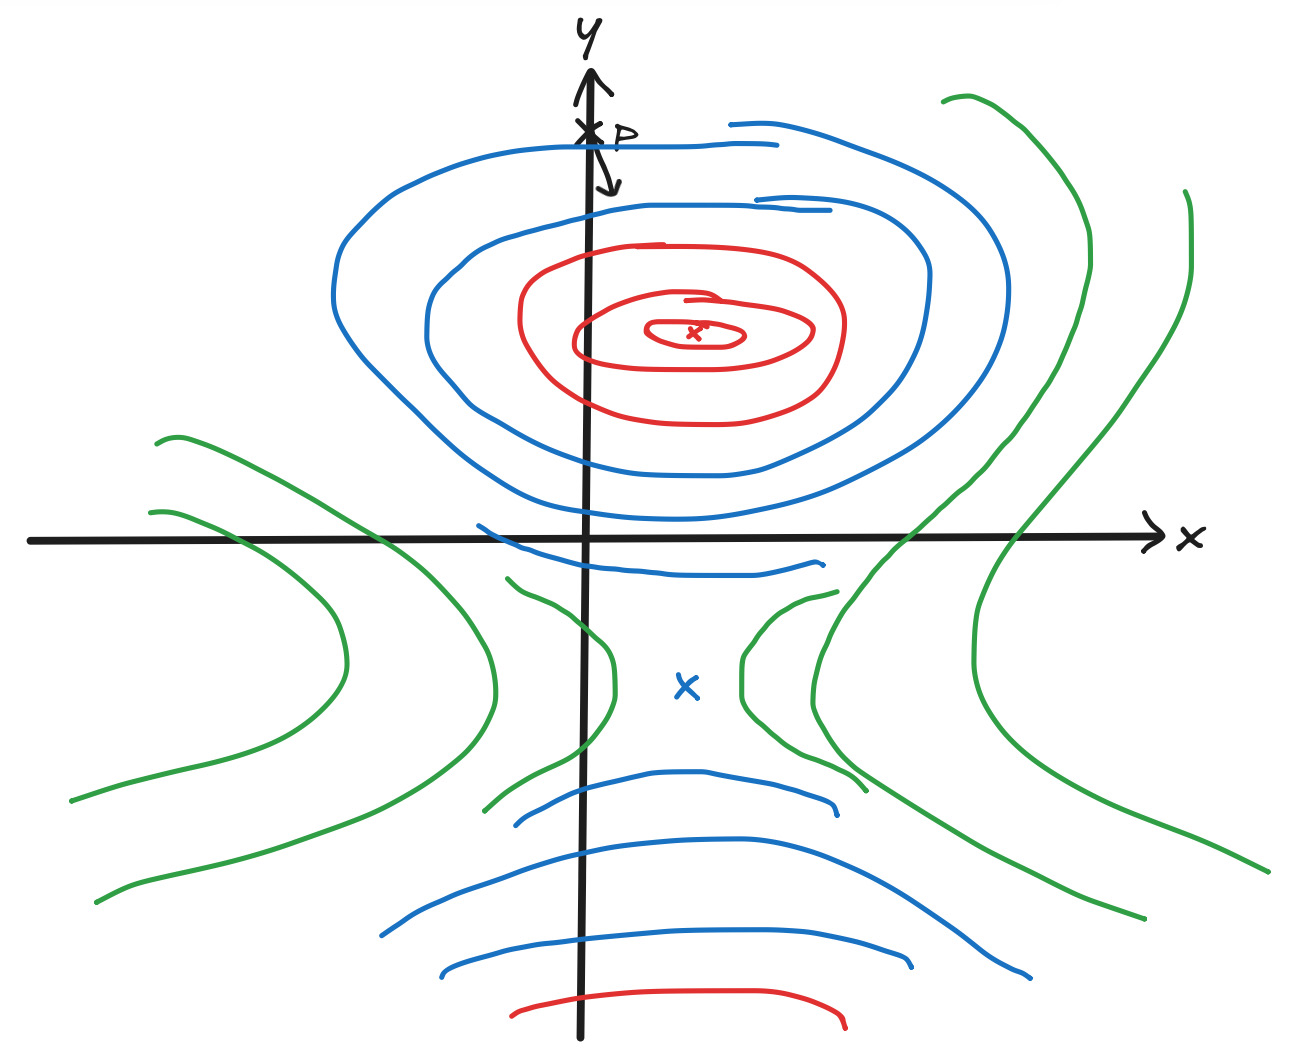
\includegraphics[scale=0.4]{Q2c}
	\caption{A contour plot of $z=f(x,y)$. Red is negative $z$, blue is small positive $z$, and green is large positive $z$. The red cross is the local minimum point, the blue cross is the saddle point, the black cross is $P$, and the black arrow is the direction of steepest descent from $P$.}
\end{figure}

\subsection{~}

\begin{figure}[h]
	\centering
	\begin{tabular}{cc}
		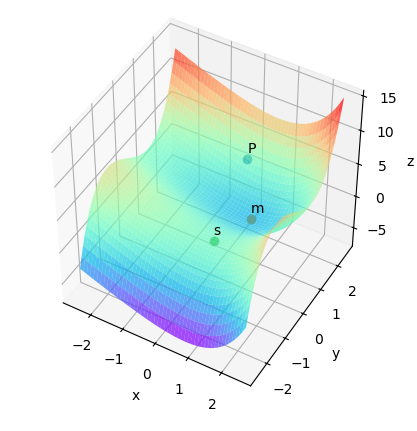
\includegraphics[scale=0.6]{Q2d-1} &
		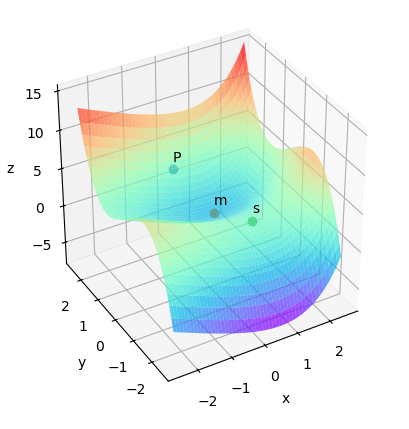
\includegraphics[scale=0.6]{Q2d-2}
	\end{tabular}
	\caption{A 3D plot of $z=f(x,y)$ from two angles. $m$ is the local minimum point and $s$ is the saddle point.}
	\label{fig:3d-plot}
\end{figure}

\begin{figure}[h]
	\centering
	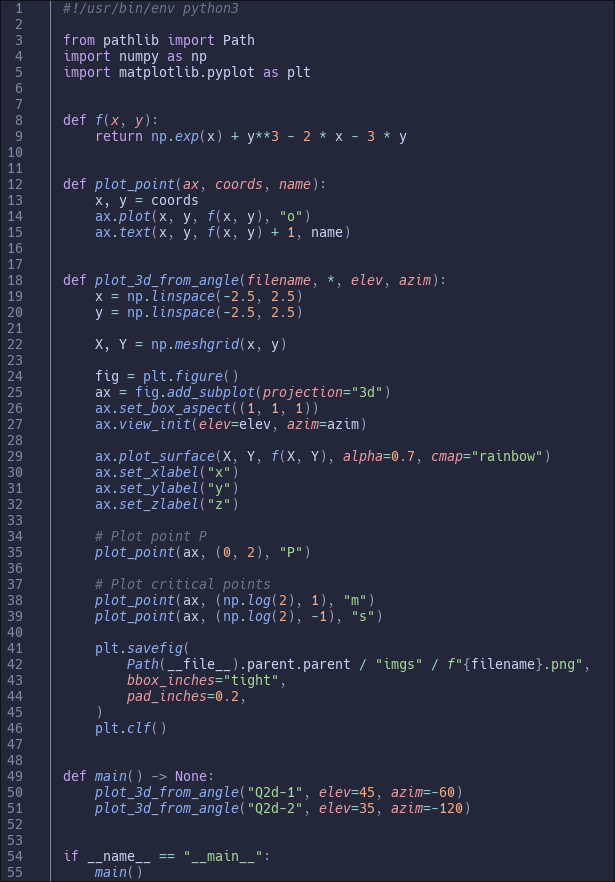
\includegraphics[scale=0.3]{Q2d-code}
	\caption{The code used to generate Figure~\ref{fig:3d-plot}. The code can also be found \href{https://github.com/DoctorDalek1963/uni/blob/1ee2e9f33bdd8e5d2054b4487684af46f686b5bd/first-year/MA144-Methods-of-Mathematical-Modelling-2/Ass 2/code/plot_surface.py}{on GitHub}.}
\end{figure}

% }}}

\end{document}
